% MIT License

% Copyright (c) 2019-2020 Simon Crase

% Permission is hereby granted, free of charge, to any person obtaining a copy
% of this software and associated documentation files (the "Software"), to deal
% in the Software without restriction, including without limitation the rights
% to use, copy, modify, merge, publish, distribute, sublicense, and/or sell
% copies of the Software, and to permit persons to whom the Software is
% furnished to do so, subject to the following conditions:

% The above copyright notice and this permission notice shall be included in all
% copies or substantial portions of the Software.

% THE SOFTWARE IS PROVIDED "AS IS", WITHOUT WARRANTY OF ANY KIND, EXPRESS OR
% IMPLIED, INCLUDING BUT NOT LIMITED TO THE WARRANTIES OF MERCHANTABILITY,
% FITNESS FOR A PARTICULAR PURPOSE AND NONINFRINGEMENT. IN NO EVENT SHALL THE
% AUTHORS OR COPYRIGHT HOLDERS BE LIABLE FOR ANY CLAIM, DAMAGES OR OTHER
% LIABILITY, WHETHER IN AN ACTION OF CONTRACT, TORT OR OTHERWISE, ARISING FROM,
% OUT OF OR IN CONNECTION WITH THE SOFTWARE OR THE USE OR OTHER DEALINGS IN THE
% SOFTWARE.

\documentclass[]{article}
\usepackage{caption,subcaption,graphicx,float,url,amsmath,amssymb,tocloft,cancel,amsthm,thmtools}
\usepackage[hidelinks]{hyperref}
\usepackage[toc,acronym,nonumberlist]{glossaries}
\usepackage{titling}
\setacronymstyle{long-short}
\usepackage{glossaries-extra}
\graphicspath{{figs/}} 
\setlength{\cftsubsecindent}{0em}
\setlength{\cftsecnumwidth}{3em}
\setlength{\cftsubsecnumwidth}{3em}
% I snarfed the next line from Stack exchange
% https://tex.stackexchange.com/questions
%    /42726/align-but-show-one-equation-number-at-the-end
% It allows me to suppress equation numbers with align*,
% then selectively add equation numbers
% for lines that I want to reference slsewhere
\newcommand\numberthis{\addtocounter{equation}{1}\tag{\theequation}}
\newtheorem{thm}{Theorem}
% Add logo at start of document


%opening
\title{
	Notes from \\
	Computation in Complex Systems
}
\author{Simon Crase (compiler)\\simon@greenweaves.nz}

\makeglossaries

\renewcommand{\glstextformat}[1]{\textbf{\em #1}}

\begin{document}

\maketitle

\begin{abstract}
   These are my notes from Computation in Complex Systems\cite{sfi2020computation}\\
   The content and images contained herein are the intellectual property of the Santa Fe Institute, with the exception of any errors in transcription, which are my own.
   These notes are distributed in the hope that they will be useful,
   but without any warranty, and without even the implied warranty of
   merchantability or fitness for a particular purpose. All feedback is welcome,
   but I don't necessarily undertake to do anything with it.\\
   \LaTeX source for the notes can be found at\\
   \url{https://github.com/weka511/complexity/tree/master/computations}.
\end{abstract}

\setcounter{tocdepth}{2}
\tableofcontents

\listoffigures
\listoftheorems[ignoreall,onlynamed]

\newglossaryentry{gls:3:SAT}{
	name={3-SAT},
	description={Given a set of \glspl{gls:clause} with 3 variables (or negated variables) each, e.g. $(x_1 \lor \bar{x_2} \lor x_3) \land (x_2 \lor x_{17} \lor \bar{x_{23}}) \land...$ is there a set $\{x_i\}$ such that all clauses are satisfied?}}

\newglossaryentry{gls:clause}{
	name={clause},
	description={In logic, a clause is an expression formed from a finite collection of literals (atoms or their negations) }}

\newglossaryentry{gls:eulerian:path}{
	name={Eulerian path},
	description={In graph theory, an Eulerian path is a path in a finite graph that visits every edge exactly once (allowing for revisiting vertices) }}

\newglossaryentry{gls:eulerian:cycle}{
	name={Eulerian cycle},
	description={Similarly, an Eulerian circuit or Eulerian cycle is an \gls{gls:eulerian:path} that starts and ends on the same vertex. }}

\newglossaryentry{gls:Hamiltonian:cycle}{
	name={Hamiltonian cycle},
	description={If a \gls{gls:Hamiltonian:path} exists whose endpoints are adjacent, then the resulting graph cycle is called a Hamiltonian cycle (or Hamiltonian cycle) }}

\newglossaryentry{gls:Hamiltonian:path}{
	name={Hamiltonian path},
	description={A Hamiltonian path, also called a Hamilton path, is a graph path between two vertices of a graph that visits each vertex exactly once }}

\newglossaryentry {gls:NAESAT} {
	name={NAESAT},
	description={An NAESAT clause is one of the form: $$
		(x_1 \lor x_2 \lor x_3) \land (\bar{x_1} \lor \bar{x_2} \lor \bar{x_3})
		$$}}
	
\newglossaryentry{gls:NonDP}{
	name={Non-deterministic Polynomial Time},
	description={we can \emph{check} a solution efficiently}}

\newglossaryentry{gls:NP:complete}{
	name={NP-Complete},
	description={It turns out that there are problems $B$ in \gls{gls:NP} such that any other problem $A$  in \gls{gls:NP} can be \gls{gls:reduced} to $B$: $A \le B \forall A \in NP$. Such a $B$ is said to be NP-Complete}}

\newglossaryentry{gls:O}{
	name={O},
	description={$f(n)=O(n^3)$ means: when $n$ is large $f(n)$ scales as $n^3$ or less. Formally:
	\begin{align*}
		f(n) =& O(g(n))\\
		\equiv&	\;\; \exists C, n_0 \text{ such that}\\
		 \forall n>n_0, f(n) \le& Cg(n)
	\end{align*}}}

\newglossaryentry{gls:o}{
	name={o},
	description={$f$ grows more slowly than $g$: $f/g \rightarrow 0 \text{ as } n\rightarrow \infty$}}

\newglossaryentry{gls:Omega}{
	name={$\Omega$},
	description={$f$ grows at least as fast as $g$: $g=O(f)$ : $f/g \cancel{\rightarrow} 0 \text{ as } n\rightarrow \infty$}}

\newglossaryentry{gls:Polynomial}{
	name={Polynomial Time},
	description={we can find a solution efficiently}}

\newglossaryentry{gls:PSPACE}{
	name={PSPACE},
	description={problems we can solve with a polynomial amout of memory, even if they take an infinire amount of time.}}

\newglossaryentry{gls:reduced}{
	name={reduced},
	description={$A$ can be \emph{reduced} to $B$, or $A \le B$, if there is a polynomial algorithm that translated instances of $A$ to instances of $B$, so the yes/no answer stays the same. }}

\newglossaryentry{gls:Theta}{
	name={$\Theta$},
	description={$f$ and $g$ grow the same way: $g=O(f)$ and $f=O(g)$ or $f/g \rightarrow C>0\text{ as } n\rightarrow \infty$}}


\newacronym[see={[Glossary:]{gls:Polynomial}}]{gls:P}{P}{Polynomial\glsadd{gls:Polynomial}}

\newacronym[see={[Glossary:]{gls:NonDP}}]{gls:NP}{NP}{Non-deterministic Polynomial\glsadd{gls:NonDP}}

\section{Easy \& Hard}

\cite[Chapters 1,2,4]{moore2011nature}

For theorists, polynomial vs. exponential is the mark of insight: we have found some structure in the problem that we can use.

\subsection{Two Kinds of Paths}

\begin{figure}[H]
	\caption{Eulerian paths}
	\begin{subfigure}[t]{0.54\textwidth}
		\caption{The 7 bridges of K\"onigsberg: can we cross each bridge only once? One strategy is brute force search.}
		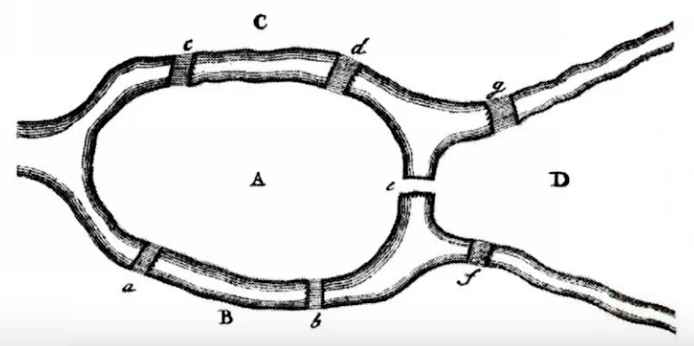
\includegraphics[width=\textwidth]{euler}
	\end{subfigure}
	\begin{subfigure}[t]{0.54\textwidth}
		\caption{Euler: if a tour exists, at most 2 noded can have an odd number of bridges, so no tour is possible. Much faster.}
		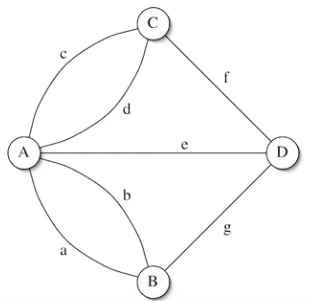
\includegraphics[width=\textwidth]{euler2}
	\end{subfigure}
\end{figure}

\begin{figure}[H]
	\begin{center}
		\caption{Hamiltonian Path: visit each node once}
		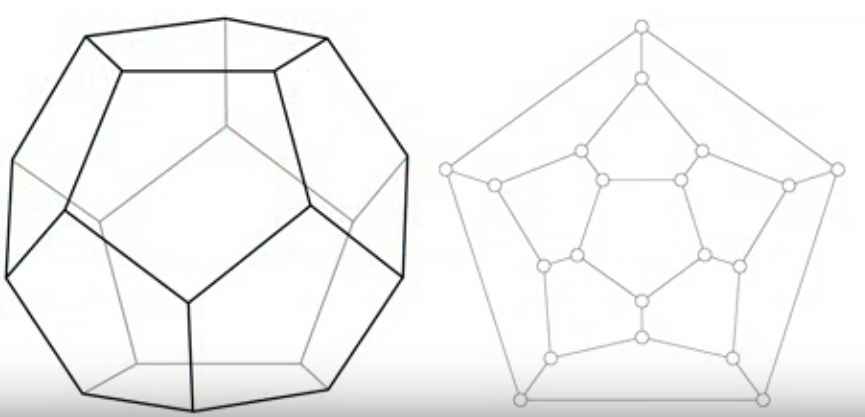
\includegraphics[width=\textwidth]{Hamiltonian}
	\end{center}
\end{figure}

\subsection{Polynomials vs. Exponentials}

Polynomials don't grow too fast Figure \ref{fig:polynomial} compared to exponential \ref{fig:exponential}.
\begin{figure}[H]
	\caption{Polynomials don't grow too fast}\label{fig:polynomial} 
	\begin{subfigure}[t]{0.3\textwidth}
		\caption{}
		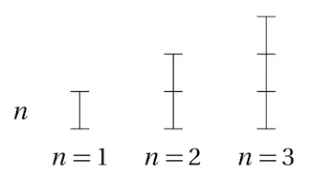
\includegraphics[width=\textwidth]{n1}
	\end{subfigure}
	\begin{subfigure}[t]{0.3\textwidth}
		\caption{}
		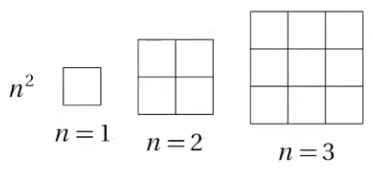
\includegraphics[width=\textwidth]{n2}
	\end{subfigure}
	\begin{subfigure}[t]{0.3\textwidth}
		\caption{}
		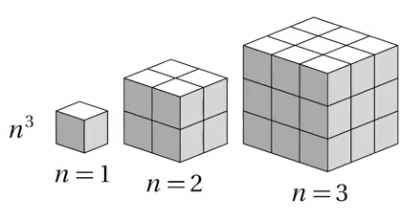
\includegraphics[width=\textwidth]{n3}
	\end{subfigure}
\end{figure}

\begin{figure}[H]
	\begin{center}
		\caption{Exponential Growth: this is what we don't want.}\label{fig:exponential}
		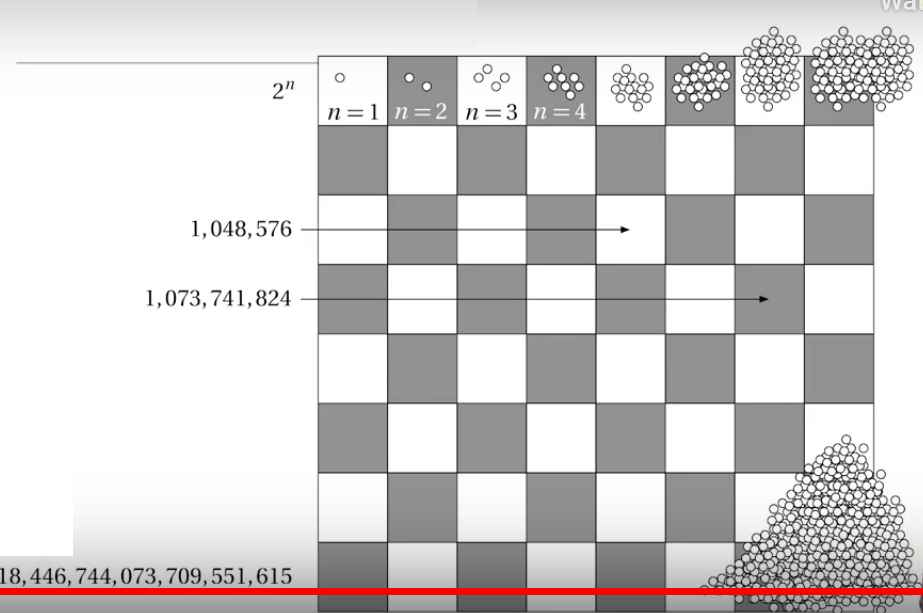
\includegraphics[width=0.8\textwidth]{exponential}
	\end{center}
\end{figure}
\subsection{Divide and Conquer}

\begin{figure}[H]
	\begin{center}
		\caption[Towers of Hanoi]{Towers of Hanoi. Figure \ref{fig:towers-hanoi-rb} shows how to break the problem--Figure \ref{fig:towers-hanoi}--down recursively.}\label{fig:toh}
		\begin{subfigure}[t]{0.35\textwidth}
			\caption{The problem}\label{fig:towers-hanoi}
			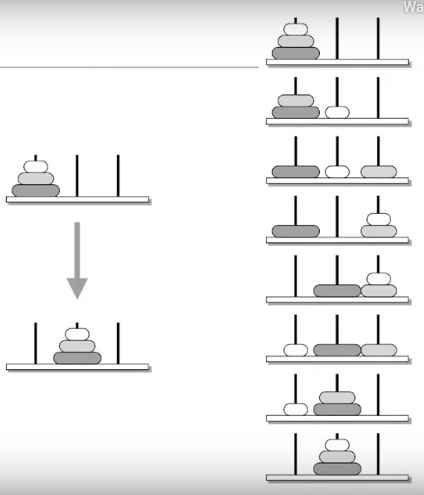
\includegraphics[width=\textwidth]{towers-hanoi}
		\end{subfigure}
		\begin{subfigure}[t]{0.6\textwidth}
			\caption{Recursive breakdown}\label{fig:towers-hanoi-rb}
			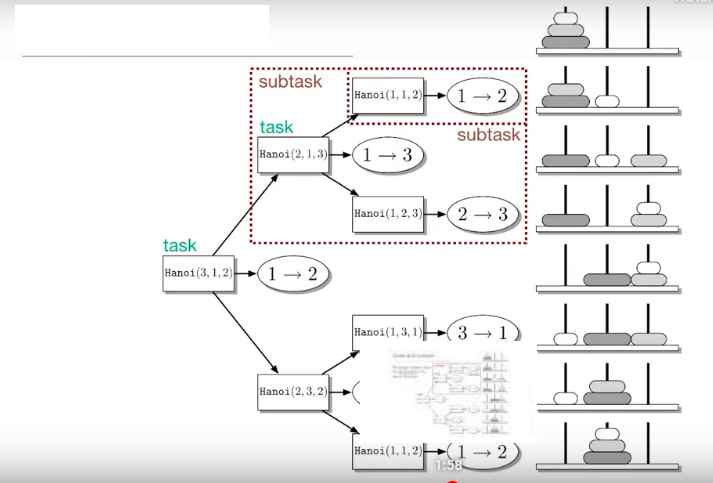
\includegraphics[width=\textwidth]{towers-hanoi-breakdown}
		\end{subfigure}
	\end{center}
\end{figure}

How many moves are needed for $n$ disks?
\begin{align*}
	f(0) =& 0 \\
	f(n) =& 2f(n-1) + 1\\
	=& 2^n -1
\end{align*}

\subsection{Big O and All that}

In computer science, a real problem is an infinite family of examples or instances. How much of some resource--time, memory, etc--do we need as a function of $n$?

\begin{itemize}
	\item \gls{gls:O} \glsdesc{gls:O}
	\item \gls{gls:Omega} \glsdesc{gls:Omega}
	\item \gls{gls:o} \glsdesc{gls:o}
	\item \gls{gls:Theta} \glsdesc{gls:Theta}
\end{itemize}

\subsection{When the details don't matter}

Polynomials vs. Exponentials.

\begin{itemize}
	\item relates to whether we can exploit some feature or are just searching;
	\item releases us from many of the details.
	\begin{itemize}
		\item The size of an instance is the number of bits to describe it, e.g. the number of bits in an email.
		\item For polynomial versus exponential, the description format doesn't matter: e.g. we can describe a network as an $n^2$ adjacency matrix, or as notes with links $n\log(n)$, but this just changes one polynomial to another.
		\item Data storage formats don't turn polynomial into exponential, e.g. linear list ($n$) versus tree ($\log(n)$) 
		\item Neither does technology--e.g. RAM vs. magnetic tape--Figure \ref{fig:imb729mtu}--$T$ vs. $T^2$.
	\end{itemize}
\end{itemize}

\begin{figure}[H]
	\begin{center}
		\caption{IBM 729 Magnetic Tape Unit}\label{fig:imb729mtu}
		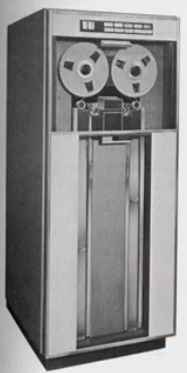
\includegraphics[width=0.6\textwidth]{imb729mtu}
	\end{center}
\end{figure}
\section{Algorithms and Landscapes}
\cite[Chapter 2]{moore2011nature}

\subsection{Divide and Conquer Redux}

How long does it take to sort a list of $n$ numbers? We could think of this as a search through $n!$ possibilities.

\begin{figure}[H]
	\caption{Mergesort: recursively split list in half, sort the halves, and merge.}\label{fig:mergesort}
	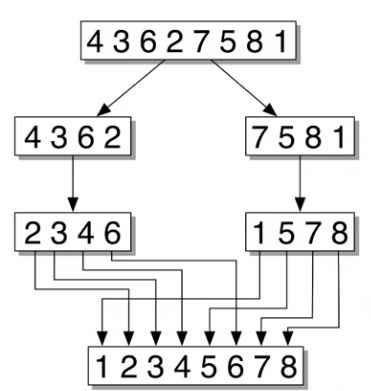
\includegraphics[width=0.8\textwidth]{mergesort}
\end{figure}

Estimate the time to sort n items by $T(n)$, the number of comparisons.
\begin{align*}
T(1) =& 0 \text{. already sorted}\\
T(n) =&\underbrace{ 2T(\frac{n}{2})}_\text{Two sorts of hald length} + \underbrace{n}_\text{Merge} \text{, hence}\\
=& n \log_2(n)
\end{align*}

\begin{table}[H]
	\begin{center}
		\caption{Number of comparisons for mergesort}
		\begin{tabular}{|r|r|} \hline
			$n$&$T(n)$  \\ \hline
			1& 0\\ \hline
			2&2 \\ \hline
			4&8 \\ \hline
			8& 24\\ \hline
			16& 64\\ \hline
			32& 160\\ \hline
		\end{tabular}
	\end{center}
\end{table}


\subsection{Dynamic Programming}

\begin{align*}
	d(s,t)=& \min(d(s^\prime,t)+1, d(s,t^\prime)+1,d(s^\prime,t^\prime) + \delta(s_1,t_1)) \text{ , where}\\
	d(s,t)=& \text{ number of changes to convert $s$ to $d$}\\
	s^\prime=& \text{ string $s$ with 1st character, $s_1$ removed}\\
	t^\prime=& \text{ string $t$ with 1st character, $t_1$ removed}
\end{align*}

There are only $n^2$ sub-problems: polynomial time.

\subsection{Greedy Algorithms}

\begin{figure}[H]
	\caption{Minimum Spanning Tree}
	\begin{subfigure}[t]{0.45\textwidth}
		\caption{e.g. power lines}
		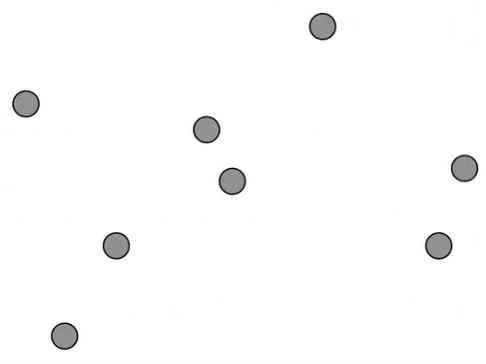
\includegraphics[width=\textwidth]{mst1}
	\end{subfigure}
	\;\;\;
	\begin{subfigure}[t]{0.45\textwidth}
		\caption{Start by adding the shortest edge}
		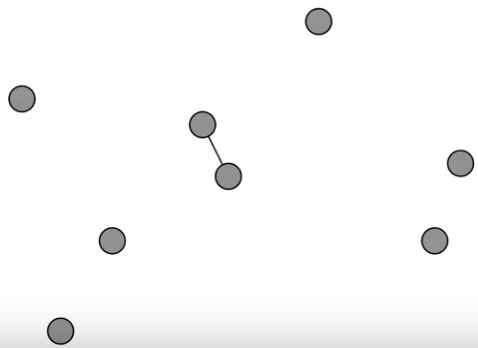
\includegraphics[width=\textwidth]{mst2}
	\end{subfigure}
	\begin{subfigure}[b]{0.45\textwidth}
		\caption{At each step, add the shortest edge that doesn't complete a cycle}
		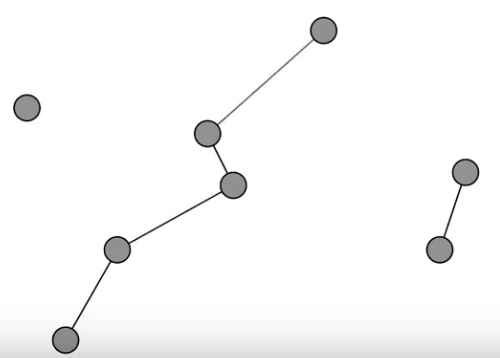
\includegraphics[width=\textwidth]{mst3}
	\end{subfigure}
	\;\;\;
	\begin{subfigure}[b]{0.45\textwidth}
		\caption{The complete tree}\label{fig:mst4}
		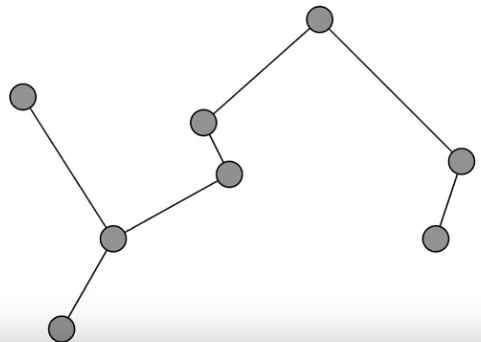
\includegraphics[width=\textwidth]{mst4}
	\end{subfigure}
\end{figure}

Clearly Figure \ref{fig:mst4} is \emph{a} spanning tree, but how do we know it is minimal?

\begin{figure}[H]
	\caption{How do we know Figure \ref{fig:mst4} is minimal?}
	\begin{subfigure}[b]{0.30\textwidth}
		\caption{Let $e$ be the shortest edge that doesn't complete a cycle, and suppose that the minimum spanning tree $T$ doesn't contain $e$}
		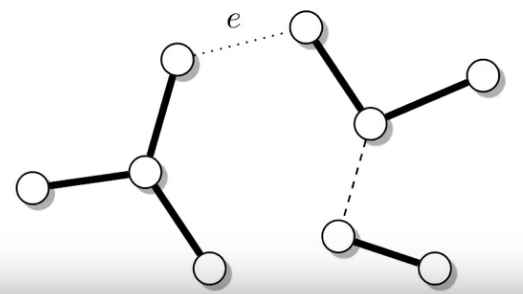
\includegraphics[width=\textwidth]{mst5}
	\end{subfigure}
	\;\;\;
	\begin{subfigure}[b]{0.30\textwidth}
		\caption{Then there must be some other path from one end of $e$ to another that goes through a longer edge $e^\prime$.}
		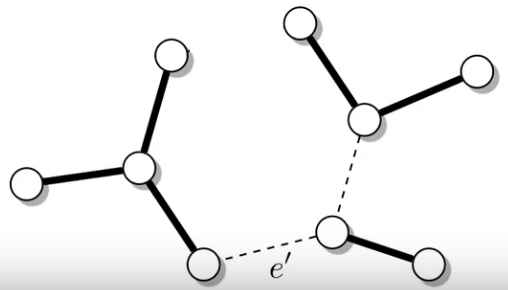
\includegraphics[width=\textwidth]{mst6}
	\end{subfigure}
	\;\;\;
	\begin{subfigure}[b]{0.30\textwidth}
		\caption{But then we could reduce the total length by deleting $e^\prime$ and adding $e$--a contradiction.}
		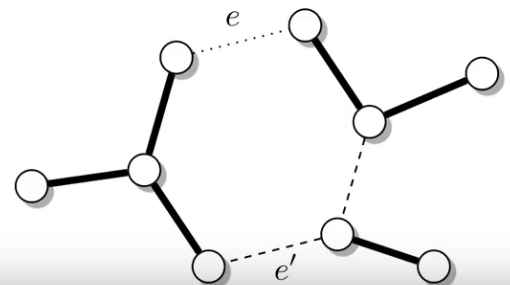
\includegraphics[width=\textwidth]{mst7}
	\end{subfigure}
\end{figure}

Greed isn't always good, or even very often good--Figures \ref{fig:greedy:tsp} and \ref{fig:lessgreedy:tsp}.
\begin{figure}[H]
	\caption{Travelling Salesman Problem}
	\begin{subfigure}[t]{0.45\textwidth}
		\caption{Greedy solution to Travelling Salesman Problem}\label{fig:greedy:tsp}
		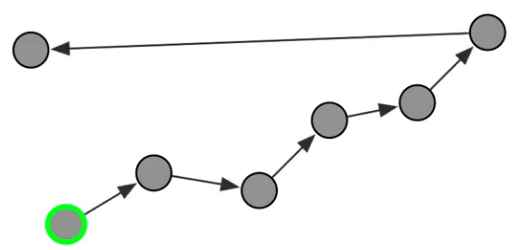
\includegraphics[width=\textwidth]{tsp1}
	\end{subfigure}
	\;\;\;
	\begin{subfigure}[t]{0.45\textwidth}
		\caption{A less Greedy solution is somewhat better}\label{fig:lessgreedy:tsp}
		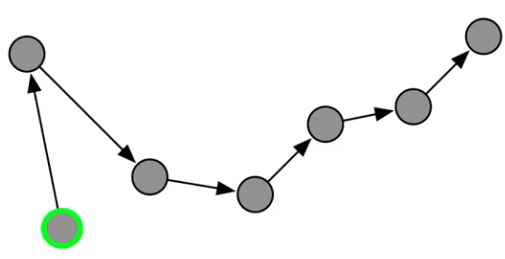
\includegraphics[width=\textwidth]{tsp2}
	\end{subfigure}
\end{figure}

\subsection{Landscapes}

\subsubsection{Greedy Algorithms and the Fitness Landscape}

\begin{figure}[H]
	\caption{Greedy Algorithms and the Fitness Landscape}
	\begin{subfigure}[t]{0.4\textwidth}
		\caption{A greedy algorithm works well if the Fitness Landscape looks like Fuji-San}
		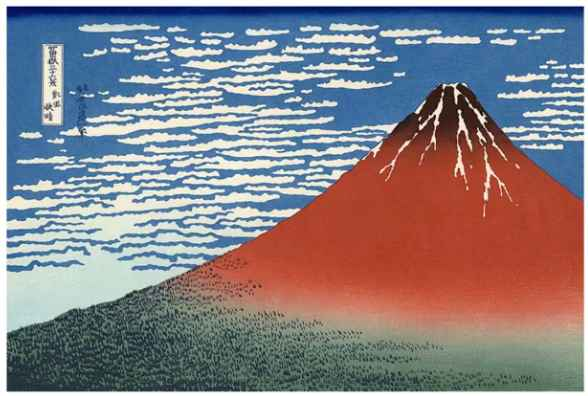
\includegraphics[width=\textwidth]{fujisan}
	\end{subfigure}
	\;\;\;
	\begin{subfigure}[t]{0.55\textwidth}
		\caption{A Greedy solution doesn't work well if there are many local optima where we can get stuck: it cannot cross a valley to get to a higher peak.}
		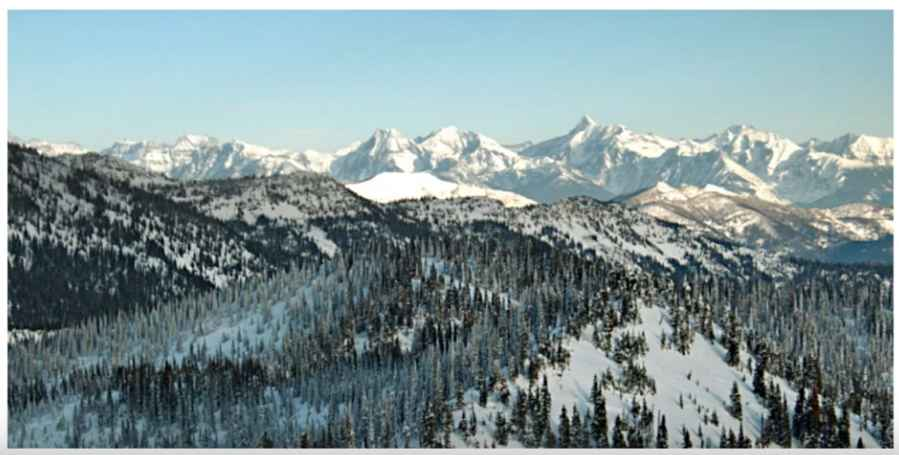
\includegraphics[width=\textwidth]{rockies}
	\end{subfigure}
\end{figure}

\subsubsection{Reorganizing the Landscape}

What defines the neighbourhood? When is one solution close to another?

\begin{figure}[H]
	\caption[Maxflow: determine the maximum flow from $s$ to $t$]{Maxflow: take a network such as \ref{fig:maxflow1} and determine the maximum flow from $s$ to $t$. We can see that we can eliminate local optima by allowing a new kind of move. By expanding our idea of what kins of solutions are neighbours we reorganize the landscape!}
	\begin{subfigure}[t]{0.4\textwidth}
		\caption{Each edge has a capacity}\label{fig:maxflow1}
		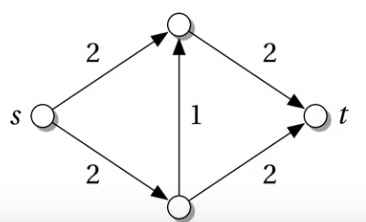
\includegraphics[width=\textwidth]{maxflow1}
	\end{subfigure}
	\;\;\;
	\begin{subfigure}[t]{0.55\textwidth}
		\caption{Greedy: push more flow along a channel with excess capacity. But we can get stuck at a local optimum. Here we have three units flowing--we are at a local optimum.}\label{fig:maxflow2}
		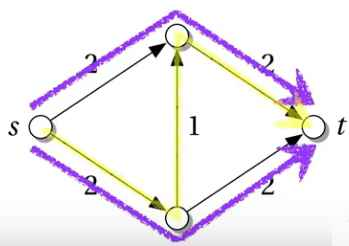
\includegraphics[width=\textwidth]{maxflow2}
	\end{subfigure}
	\;\;\;
	\begin{subfigure}[t]{0.45\textwidth}
		\caption{We should have done this instead}\label{fig:maxflow3}
		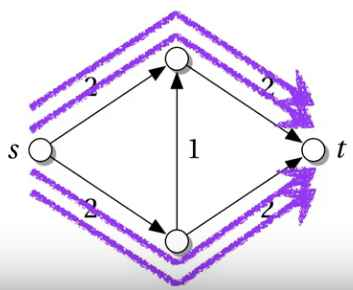
\includegraphics[width=\textwidth]{maxflow3}
	\end{subfigure}
	\;\;\;
	\begin{subfigure}[t]{0.45\textwidth}
		\caption{Allow reverse edges to cancel previous flow: now if we add to Figure \ref{fig:maxflow2} we get the optimum--Figure \ref{fig:maxflow3}. If we allow this type of move we can never get stuck: there are no local optima.}
		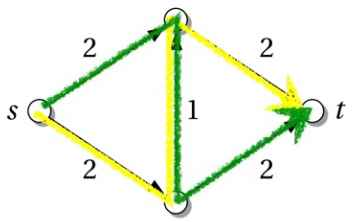
\includegraphics[width=\textwidth]{maxflow4}
	\end{subfigure}
\end{figure}

This won't always work. Some problems are inherently bumpy.

\subsection{Reductions and Translations}

\begin{figure}[H]
	\caption[Reducing one problem into another]{Reducing one problem into another. We want a perfect bipartite matching, where everyone has a partner. This is a subset of the edges of this graph, so everyone on one side is connected to exactly one person on the other. There are $n!$ possible matchings.}
	\begin{subfigure}[t]{0.3\textwidth}
		\caption{Bipartite Graph. }
		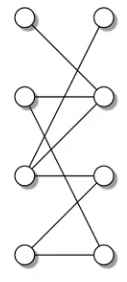
\includegraphics[width=\textwidth]{bpg1}
	\end{subfigure}
	\;\;\;
	\begin{subfigure}[t]{0.65\textwidth}
		\caption{We can transform the problem to max flow. Each compatible couple becomes an edge with flow 1.}
		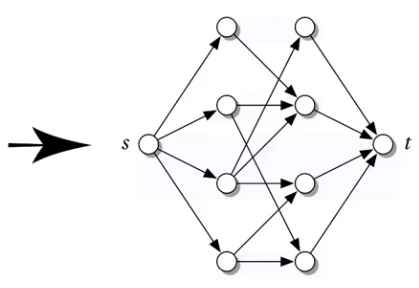
\includegraphics[width=\textwidth]{bpg2}
	\end{subfigure}
\end{figure}

\begin{thm}[Maxflow]
	If all the flows have integral capacities, the solution is also integral.
\end{thm}

In terms of complexity, Bipartite Matching $\le$ Max Flow.


\begin{figure}[H]
	\caption{Shortest Path}
	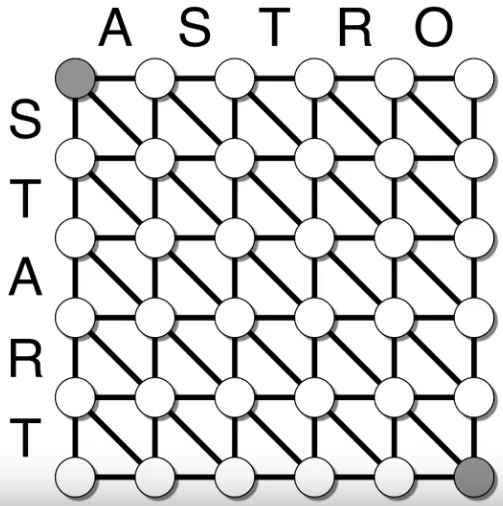
\includegraphics[width=0.8\textwidth]{sp1}
\end{figure}

\subsection{Lessons So Far}

We have just a few techniques that are guaranteed to be efficient:
\begin{itemize}
	\item divide and conquer;
	\item dynamic programming;
	\item greedy (local search);
	\item linear programming, convex programming and duality (max-flow and min-cut).
\end{itemize}
These are essentially all we know about: is that all there is?

\subsection{The Best of All Possible Algorithms}

How do we know whether an algorithm is optimal? How long does it take to multiply two $n$ digit numbers? The algorithm we learned in primary school takes time $\propto n^2$. 

\begin{figure}[H]
	\begin{center}
		\caption{What if we try divide and conquer?}
		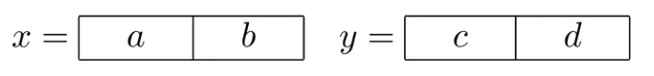
\includegraphics[width=0.6\textwidth]{dc-mult}
	\end{center}
\end{figure}

\begin{align*}
	x=& 10^\frac{n}{2}a+b\\
	y =& 10^\frac{n}{2}c+d\\
	xy=& 10^n a c + 10^\frac{n}{2}(ad+bc) + bd \numberthis \label{eq:xy}
\end{align*}
Multiplication is typically slower than add and shifting. We replace one multiplication of $n$ digit numbers with 4 multiplications of $\frac{n}{2}$ numbers: $T(n) \approx 4T(\frac{n}{2})$. But maybe we can be a bit more clever.

\begin{align*}
	(a+b)(c+d) -ac -bd =& ad+bc 
\end{align*}

We can evaluate (\ref{eq:xy}) with only 3 multiplications, and the running time is now governed by $T(n) \approx 3T(\frac{n}{2})$.

We will solve the equation for T.
\begin{align*}
	T(n) =&3T(\frac{n}{2}) \text{, we want a solution of the form}\\
	T(n) \propto& n^\alpha \text{, whence}\\
	\cancel{n}^\alpha =& 3\big(\frac{\cancel{n}}{2}\big)^\alpha\\
	2^\alpha =& 3\\
	\alpha \log(2) =& \log(3)\\
	\alpha =& \frac{\log(3)}{\log(2)}\\
	\approxeq& 1.585\\
	T(n) \propto n^{1.585} 
\end{align*}
It turns out that we can get $\alpha$ down as close to 1 as we want.

How does mergesort $n \log_2(n)$ compare with best possible algorithm? Figure \ref{fig:dt-sort} illustrates the decision table for searching. There needs to be  $\log_2(n!) \approx n \log_2(n)$ comparisons: merge sort is about as good as it gets.

\begin{figure}[H]
	\begin{center}
		\caption{Decision Table for Sort}\label{fig:dt-sort}
		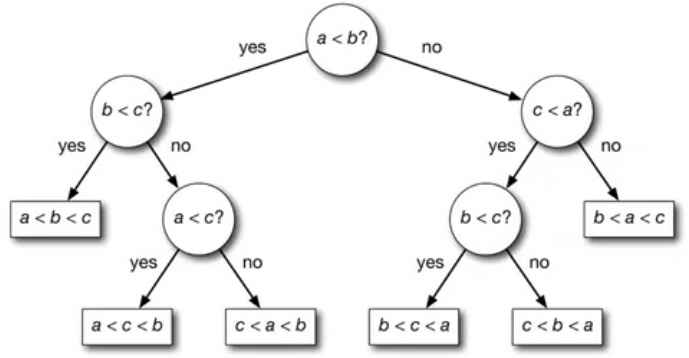
\includegraphics[width=0.6\textwidth]{dt-sort}
	\end{center}
\end{figure}

\subsection{Complexity Wrap-Up}

\begin{itemize}
	\item \emph{Systems} aren't simple or complex; questions about them are.
	\item Intrinsic complexity of a problem: the running time, or memory, or other resource, of the \emph{best possible algorithm}; an objective mathematical fact.
	\item Upper bounds are easy: just give an algorithm.
	\item Lower bounds are hard.
	\item Lower bounds show that one problem is at least as easy (or hard) as another. 
\end{itemize}

\section{P versus NP}
\cite[Chapters 4-6]{moore2011nature}, \cite{sep-computability}

\subsection{Finding versus Checking}

Some problems can be solved in polynomial time, while other require a brute-force search, which is typically exponential. In the P vs. NP question we deal with ''needles in haystacks'': finding a solution, or telling whether there is one seems hard, by checking a solution is easy.

\begin{figure}[H]
	\begin{center}
		\caption[Hamiltonian path]{\gls{gls:Hamiltonian:path}. We don't know how to solve it in polynomial time, but we can easily check a proposed solution.}\label{fig:PNP1}
		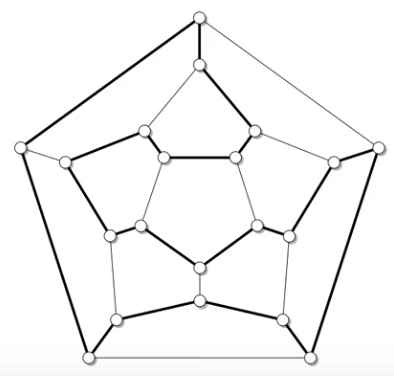
\includegraphics[width=0.8\textwidth]{PNP1}
	\end{center}
\end{figure} 

\begin{itemize}
	\item \gls{gls:P}: \glsdesc{gls:Polynomial}
	\item \gls{gls:NP}: \glsdesc{gls:NonDP}
\end{itemize}

\begin{figure}[H]
	\begin{center}
		\caption[Complexity Classes]{Complexity Classes. We \emph{know} that $P \subseteq NP$, and we \emph{believe} that $P \subset NP$}\label{fig:PNP2}
		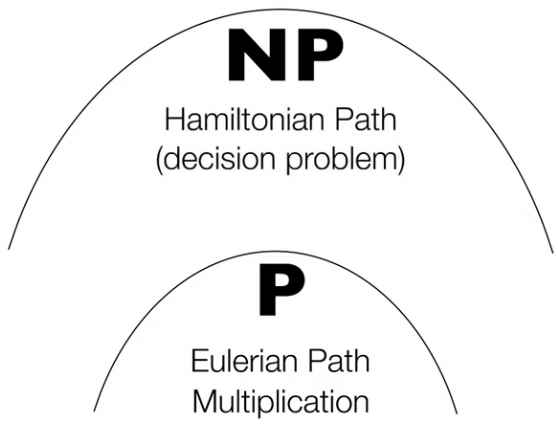
\includegraphics[width=0.8\textwidth]{PNP2}
	\end{center}
\end{figure}

We'll focus on classes of decision problems: not \emph{does this graphs have a \gls{gls:Hamiltonian:path}}, but \emph{can we find a \gls{gls:Hamiltonian:path} for \emph{\gls{gls:Hamiltonian:path}} graph}. We consider \gls{gls:NP:complete} problems.

We say that \glsdesc{gls:reduced} \glsdesc{gls:NP:complete}

But if $A \le B$ and $A$ is hard, them $B$ must be hard too: so $B$ is one of the hardest problems in \gls{gls:NP}. We can therefore focus on one  \gls{gls:NP}: if $B\in NP$ we would know that $P=NP$. Conversely, if $P \ne NP$, $B$ cannot be solved in polynomial time.

Now the Hamiltonian Path problem is NP-Complete: how can such a simple problem represent all \gls{gls:NP} problems?

\subsection{Circuits and Formulae}

Figure \ref{fig:satisfying} illustrates how the question ''is there a \gls{gls:Hamiltonian:path}'' can be transformed to ''are there values for the inputs that make to output \textbf{true}?''
\begin{figure}[H]
	\begin{center}
		\caption{Satisfying a circuit}
		\begin{subfigure}[b]{0.45\textwidth}
			\caption{Satisfying a circuit: any program that tests solutions--e.g. to \gls{gls:Hamiltonian:path}--can be compiled into a Boolean circuit--bits!}\label{fig:satisfying}
			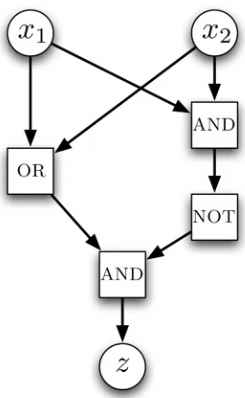
\includegraphics[width=\textwidth]{satisfy}
		\end{subfigure}
		\begin{subfigure}[b]{0.45\textwidth}
			\caption{Add variables representing the truth values of the wires.}\label{fig:add:variables}
			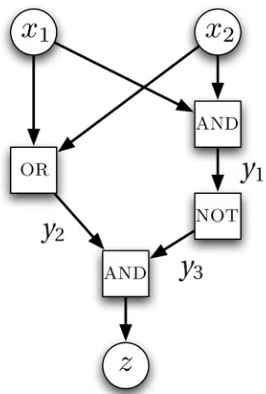
\includegraphics[width=\textwidth]{add-variables}
		\end{subfigure}
	\end{center}
\end{figure}

\begin{align*}
	y = x_1 \land& x_2 \equiv (x_1\lor \bar{y_1}) \land (x_1\lor \bar{y_2}) \land (\bar{x_1} \lor \bar{x_2} \lor y_1)
\end{align*}

We have converted the problem of checking a problem to a program, and than into a problem of checking Boolean expressions. We have therefore reduced out original problem to an instance of \gls{gls:3:SAT}, one of the original 6 \gls{gls:NP:complete} problems.
\glsdesc{gls:3:SAT} k-SAT is ($k$ variables per clause) is \gls{gls:NP:complete} $\forall k \ge 3$.

If \gls{gls:3:SAT} were easy:
\begin{itemize}
	\item we could take any \gls{gls:NP} problem;
	\item write a program that checks a solution;
	\item convert to a circuit;
	\item convert to a 3-SAT formula;
	\item use our efficient 3-SAT solver to solve the original problem;
	\item so if $3-SAT \in P$ then $P=NP$.
	\item If $P\ne NP$, 3-SAT cannot be solved in polynomial time.
\end{itemize}

\begin{thm}[k-SAT $\le$ 3-SAT]
	k-SAT $\le$ 3-SAT
\end{thm}

\begin{proof}
	We can break k-clauses down into 3-clauses, by adding new variables $\{z_i\}$, e.g.:
	\begin{align*}
		(x_1 \lor x_2 \lor x_3 \lor x_4 \lor x_5) =& (x_1 \lor x_2 \lor z_1) \land (\bar{z_1} \lor x_3 \lor z_2) \land (\bar{z_2} \lor x_4 \lor x_5)
	\end{align*}
	so we get 3-SAT clauses. They are good logical building blocks: this isn't true for 2-SAT clauses. A 3-SAT clause has ''chemistry'' and triggers a search. 
\end{proof}

\begin{thm}[2-SAT $\in$ P.]
	2-SAT $\in$ P.
\end{thm}

\begin{proof}
	TBP
\end{proof}

\subsection{More NP-complete Problems}

\begin{itemize}
	\item Polynomial time reduction is transitive: $A \le B \land B \le C\implies A \le C$.
	\item So we can prove a problem is NP-complete by reducing any other problem to it.
	\item e.g. Circuit satisfiability $\le$ 3-SAT.
	\item 3-SAT $\le$ \gls{gls:NAESAT}--\glsdesc{gls:NAESAT}
\end{itemize}

\subsubsection{Not All Equal SAT}

We need to be careful when we reduce to know which direction we are going.
Can we build \gls{gls:3:SAT} out of \gls{gls:NAESAT} building blocks?
\begin{itemize}
	\item \gls{gls:3:SAT} is symmetric: can we build it out of asymmetric parts?
	\item Add a global variable $s$ to break the symmetry.
	\item Consider the NAE-4-SAT clause $(x_1,x_2,x_3,s)$: what if $s$ false? what if it is true?
	\item This translates  \gls{gls:3:SAT} to NAE-4-SAT. Then we can use the same trick we used above for k-SAT to reduce  NAE-4-SAT to NAE-3-SAT.
\end{itemize}

\subsubsection{Map Colouring Problem}
\begin{figure}[H]
	\begin{center}
		\caption[Map Colouring Problem]{Given a map of countries and borders between them,what is the smallest number of countries we need?}\label{fig:MapColouring}
		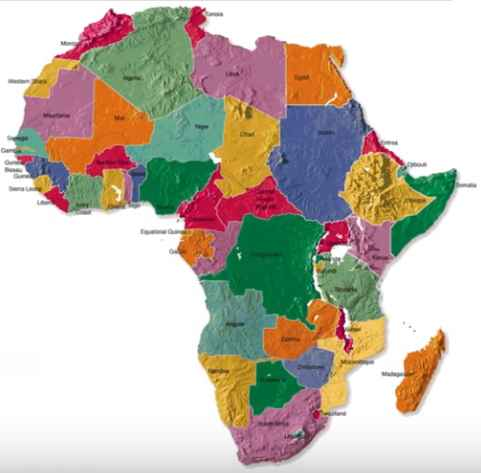
\includegraphics[width=0.8\textwidth]{MapColouring}
	\end{center}
\end{figure}

We know that 4 colours are enough: it turns out that the 3-Colour problem is \gls{gls:NP:complete}--Figure \ref{fig:naesat3colour}.
\begin{figure}[H]
	\caption[NAESAT $\le$ Graph 3-Colour]{NAESAT $\le$ Graph 3-Colour: each node is a country, and each border an edge; two nodes are connected \emph{iff} the two countries share a border.}\label{fig:naesat3colour}
	\begin{subfigure}[t]{0.45\textwidth}
		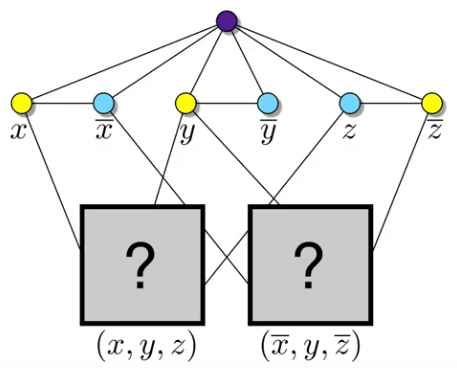
\includegraphics[width=0.8\textwidth]{naesat3colour}
	\end{subfigure}
	\begin{subfigure}[t]{0.45\textwidth}
		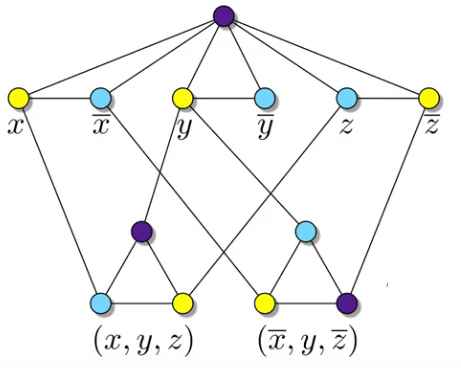
\includegraphics[width=0.8\textwidth]{naesat3solution}
	\end{subfigure}
\end{figure}

\begin{thm}[NAESAT $\le$ Graph 3-Colour]
	NAESAT $\le$ Graph 3-Colour
\end{thm}

\begin{proof}
	\begin{enumerate}
		\item Use gadgets to encode variables and enforce constraints.
		\item If there are two ways to colour something we call the colours ''true'' and ''false''--e.g. the triangles at the top.
		\item Assign an arbitrary colour to the topmost node.
		\item TBP
	\end{enumerate}
\end{proof}

3 colouring can be a disguise for any search problem--Hamiltonian path, TSP,...

\subsection{P versus NP Problem}

If any NP problem can be solved in polynomial time, then they all can, and $P=NP$. This would mean that any problem that is easy to check would also be easy to find.

The question is still open, because we don't know all the possible ways to solve problems in polynomial time.

P and NP is about the nature of mathematical truth and creativity.

\subsection{Existence and Nonexistence }

A yes/no question is in NP if, whenever the answer is "yes", there is an easily checked proof or "witness" to that fact. Note there is an asymmetry, as we don't have to worry about "No". 

\subsection{Above and Beyond}

The class NP is about the existence of things: if it exists, and it is easy to check if you show it to me, then its in NP. As we go to deeper and more tangled relationships we find ourselves climbing through an infinite hierarchy--Figure \ref{fig:complexity:hierarchy}.

\begin{figure}[H]
	\caption{Complexity Hierarchy}\label{fig:complexity:hierarchy}
	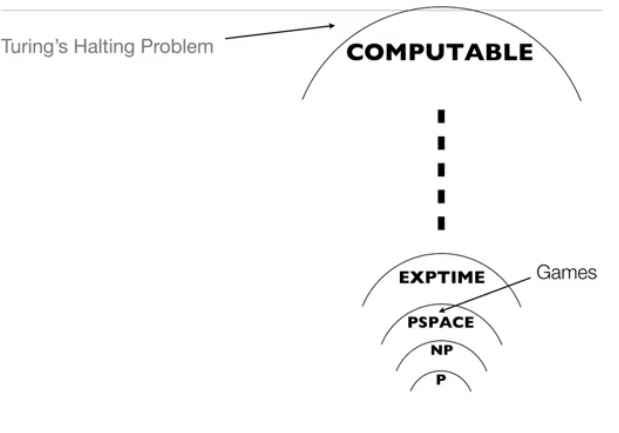
\includegraphics[width=0.8\textwidth]{hierarchy}
\end{figure}

Strategies are larger than Hamiltonian Paths: to prove that one side has a winning strategy I need to check an exponential path--Figure \ref{fig:PSPACE}. Playing games perfectly lives higher up in the complexity hierarchy--Figure \ref{fig:complexity:hierarchy}. 
\begin{figure}[H]
	\begin{center}
		\caption{Strategies are larger than Hamiltonian Paths}\label{fig:PSPACE}
		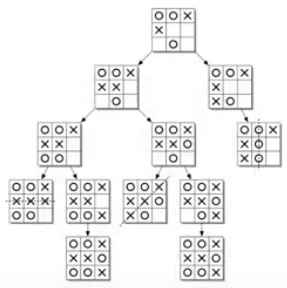
\includegraphics[width=0.6\textwidth]{PSPACE}
	\end{center}
\end{figure}

Exploring the tree could take exponential time, but, if the length of the game is polynomial, we only need polynomial space. We have another complexity class: \gls{gls:PSPACE}--\glsdesc{gls:PSPACE}

\begin{thm}
	$P \subseteq NP \subseteq PSPACE$
\end{thm}

\begin{proof}
	TBP
\end{proof}

We have a language to draw qualitative distinctions between problems, to locate them in the hierarchy of--Figure \ref{fig:complexity:hierarchy}.
\begin{quotation}
	Computers play the same role in complexity that clocks, trains, and elevators play on relativity--Scott Aaronson.
\end{quotation}

Computer science is not the study of computers, it is the study of computation.

\begin{figure}[H]
	\begin{center}
		\caption[Rule 110 is universal]{Rule 110 is universal\cite{cook2004universality}}
		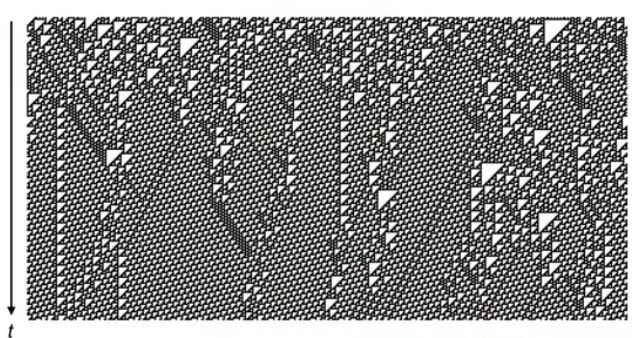
\includegraphics[width=0.8\textwidth]{rule110}
	\end{center}
\end{figure}

Given a cellular automaton, what questions can we ask about it?

\begin{enumerate}
	\item What will the state be at $t_{n+x}$?

	\item Does s have a predecessor?

	\item On a lattice of size $n$, is $s$ on a periodic orbit?

	\item On a lattice of infinite size, will $s$ ever die out?
	
\end{enumerate}

These all live at different levels of Figure \ref{fig:complexity:hierarchy}.

\section{Worst-case, Natural, and Random}
\cite[Chapters 5,10]{moore2011nature}

\subsection{Real World Problems}

There are some gaps or bridges to cross between this theory and real world problems. \gls{gls:NP:complete}ness is a worst-case notion. Computer science assumes that instances are designed by a clever adversary to encode hard problems. For example, we showed that we could design a particularly hard graph colouring problem; this is good in cryptography, but not necessary in science. The solution to many physics problems are the simplest, most optimistic equation.

\begin{quote}
	The scientist is always working to discover the order and organization of the universe, and is thus playing a game against the arch enemy, disorganization. Is this devil Manichaean or Augustininan? Is it a contrary force opposed to order or is it the very absence of order itself?--Norbert Wiener, Cybernetics.
\end{quote}

Many algorithms that take exponential time in the worst case are efficient in practice.
Linear programming problems are a large class of optimization problems that include max flow and min cut. Solving them is like climbing to the top of a high dimensional jewel. There is an old algorithm, the simplex method, which is a simple greedy algorithm. People have dreamed up problems where the simplex method is exponential, but, in practice, real problems are typically tractable.

Spielman and Teng\cite{spielman2004smoothed} realized that noise foils the adversary, making a smoother problem: the number of facets goes down, and the path to the top get shorter. In the real world you never know the coefficients exactly, you never know exactly what the right hand side is. In the real world things are a wee bit noisy. Spielman and Teng observed that adding noise almost always makes the problem simpler. It greatly reduces the number of vertices on the path to the top, so the simplex algorithm will work efficiently (almost always).

\begin{figure}[H]
	\begin{center}
		\caption{Smoothed Analysis}\label{fig:hs-jewel}
		\begin{subfigure}[t]{0.45\textwidth}
			\caption{Optimization problems are like exploring a high dimensional jewel}
			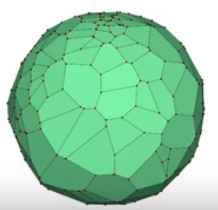
\includegraphics[width=\textwidth]{hs-jewel}
		\end{subfigure}
		\begin{subfigure}[t]{0.45\textwidth}
			\caption{Noise foils the adversary}
			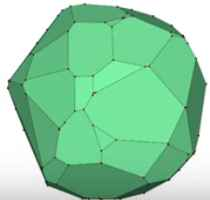
\includegraphics[width=\textwidth]{hd-jewel2}
		\end{subfigure}
	\end{center}
\end{figure}

There are hard examples of this problem, but they are rare and they are fragile. The adversary has to fine-tune the problem to make it hard. But there are other problems where we think hard problems are common and robust--e.g. cryptosystems.

Some real world problems are easy because of the structure of the landscape.

If you define clustering as optimization it is a hard problem, but it is one we solve every day. Why? Because of local minima. Maybe we are asking the wrong question: if there is one true clustering, it should be shouting at us, and there should not be other clustering that are almost as good but very different.

\begin{figure}[H]
	\caption{Landscapes are not as bumpy as they could be: if all good solutions are close to the optimum, cluster is easy. But if the landscape is really bumpy, maybe the pattern that we are looking for isn't really there.}\label{fig:rw-problems-easy}
	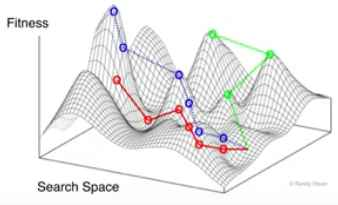
\includegraphics[width=0.6\textwidth]{rw-problems-easy}
\end{figure}

Suppose the instance in front of you has the following structural property to its landscape of solutions:suppose that any local optimum that is almost as good as the global optimum is also close to the global optimum and agrees with it on most points. So there might be local foothills to the global optimum, but the global optimum dominates the landscape: you don't have another peak far away that is almost as high. Under this structural assumption Balcan, Blum and Gupta\cite{balcan2013clustering} showed that a certain clustering algorithm, similar to the k-means algorithm works very well and very quickly.

Another example of why real-world problems might be easy is protein folding. We have co-evolved the  sequences and the algorithms. If you look at energy, there is a nice deep bowl surrounding the correct conformation. Organism that live at higher temperatures have deeper bowls so the proteins won't accidentally get kicked out. 

So real world problems mostly have nicer landscapes than we'd expect from a diabolical adversary.
  
\subsection{Phase Transitions}

\subsection{Random Problems}

\subsection{Solvability Threshold}

\subsection{Modeling Differential Equations}

\subsection{Landscapes, Clustering, Freezing, and Hardness }


\section{Computation Everywhere}
\cite[Chapter 7]{moore2011nature}
% end of text 

% glossary

\printglossaries

% bibliography go here
 
\bibliographystyle{unsrt}
\addcontentsline{toc}{section}{Bibliography}
\bibliography{computations}

\end{document}
